\documentclass[tikz,border=4pt]{standalone}
% Estilos compartilhados pelos diagramas dos estágios e módulos do Core.
\usetikzlibrary{arrows.meta, positioning, calc, shapes.geometric, fit}

\tikzset{
  >={Stealth[length=2.2mm]},
  bloco/.style={draw, rounded corners=2pt, minimum width=24mm, minimum height=9mm,
                align=center, font=\small, fill=blue!6},
  regpipe/.style={draw, minimum width=9mm, minimum height=48mm, align=center,
                  font=\small, fill=gray!25},
  mux/.style={draw, trapezium, trapezium angle=70, shape border rotate=90,
              minimum height=11mm, minimum width=7mm, inner sep=1pt, align=center,
              font=\scriptsize, fill=orange!15},
  ctrl/.style={draw, rounded corners=2pt, minimum width=24mm, minimum height=9mm,
               align=center, font=\small, fill=green!10},
  opcional/.style={bloco, dashed, fill=yellow!12},
  externo/.style={draw, rounded corners=2pt, minimum width=24mm, minimum height=9mm,
                  align=center, font=\small, fill=red!8},
  dado/.style={->, thick},
  sinal/.style={->, dashed},
  rotulo/.style={font=\scriptsize, midway, above, inner sep=1pt},
  titulo/.style={font=\bfseries\normalsize}
}

\begin{document}
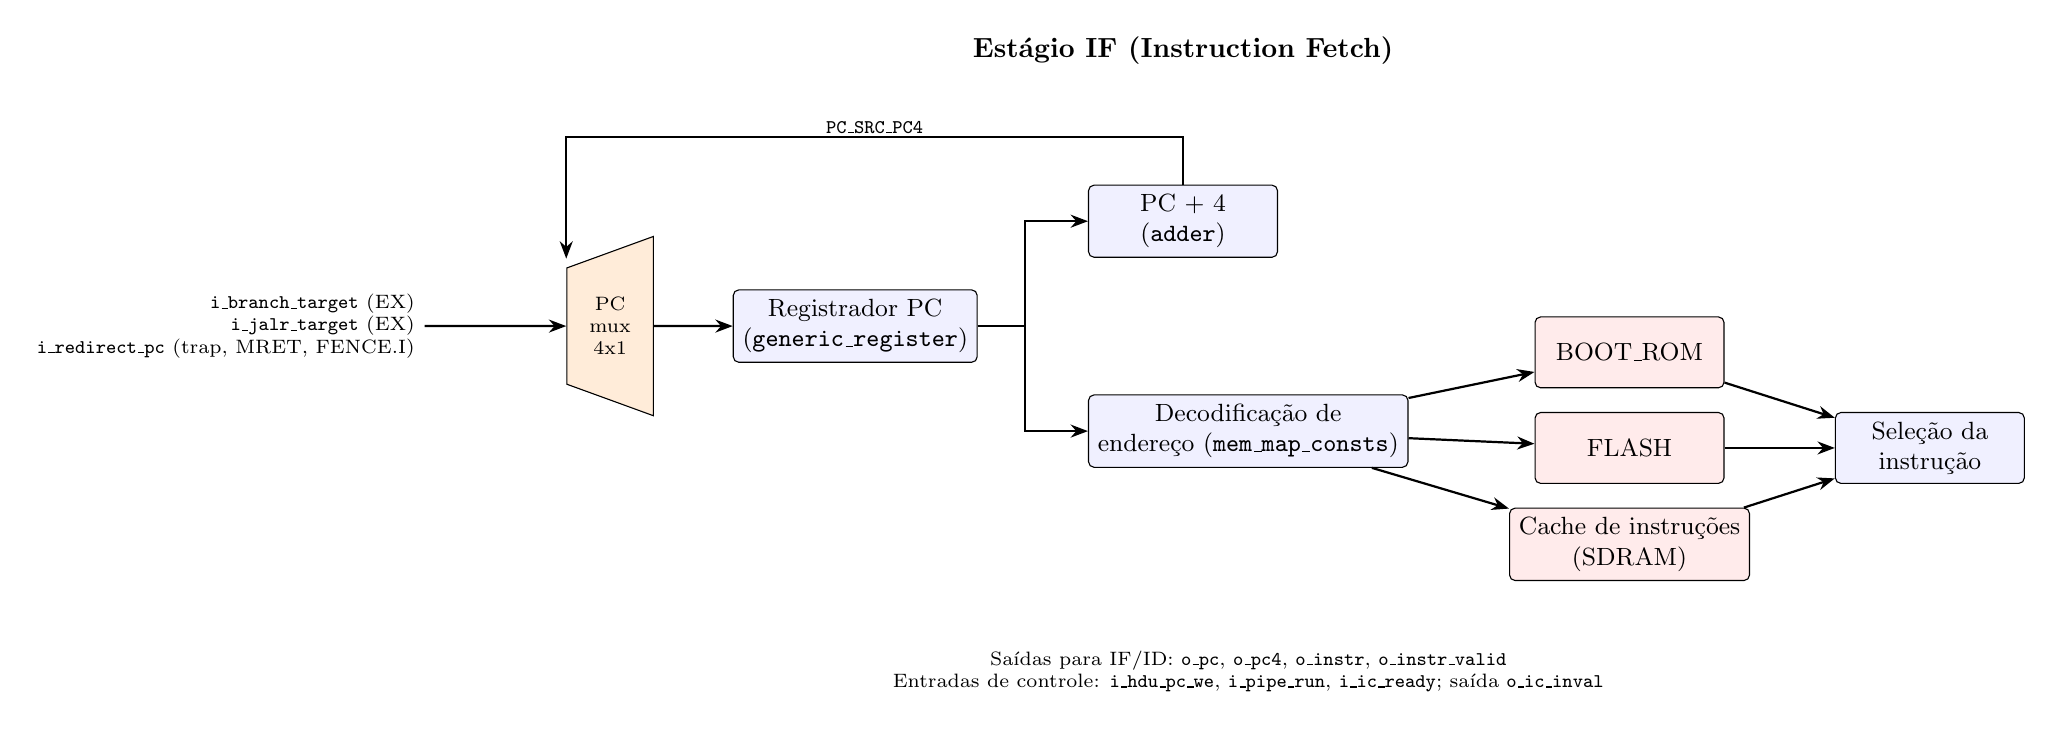
\begin{tikzpicture}[node distance=9mm and 14mm]
  \node[mux] (pcmux) {PC\\mux\\4x1};
  \node[bloco, right=10mm of pcmux] (pcreg) {Registrador PC\\(\texttt{generic\_register})};
  \node[bloco, above right=4mm and 14mm of pcreg] (add) {PC + 4\\(\texttt{adder})};
  \node[bloco, below right=4mm and 14mm of pcreg] (dec) {Decodificação de\\endereço (\texttt{mem\_map\_consts})};
  \node[externo, right=16mm of dec, yshift=10mm] (boot) {BOOT\_ROM};
  \node[externo, below=3mm of boot] (flash) {FLASH};
  \node[externo, below=3mm of flash] (ic) {Cache de instruções\\(SDRAM)};
  \node[bloco, right=14mm of flash] (isel) {Seleção da\\instrução};

  \draw[dado] (pcmux) -- (pcreg);
  \draw[dado] (pcreg.east) -- ++(6mm,0) |- (add.west);
  \draw[dado] (pcreg.east) -- ++(6mm,0) |- (dec.west);
  \draw[dado] (add.north) -- ++(0,6mm) -| node[rotulo,pos=.25] {\texttt{PC\_SRC\_PC4}} ([yshift=3mm]pcmux.north west);
  \draw[dado] (dec) -- (boot);
  \draw[dado] (dec) -- (flash);
  \draw[dado] (dec) -- (ic);
  \draw[dado] (boot) -- (isel);
  \draw[dado] (flash) -- (isel);
  \draw[dado] (ic) -- (isel);

  \node[left=18mm of pcmux, align=right, font=\scriptsize] (srcs)
    {\texttt{i\_branch\_target} (EX)\\\texttt{i\_jalr\_target} (EX)\\\texttt{i\_redirect\_pc} (trap, MRET, FENCE.I)};
  \draw[dado] (srcs) -- (pcmux);

  \node[font=\scriptsize, below=22mm of dec, align=center] (sai)
    {Saídas para IF/ID: \texttt{o\_pc}, \texttt{o\_pc4}, \texttt{o\_instr}, \texttt{o\_instr\_valid}\\
     Entradas de controle: \texttt{i\_hdu\_pc\_we}, \texttt{i\_pipe\_run}, \texttt{i\_ic\_ready}; saída \texttt{o\_ic\_inval}};
\node[titulo, above=14mm of add] {Estágio IF (Instruction Fetch)};
\end{tikzpicture}
\end{document}
